\section{Tests de robustesse et de performances}

\subsection{Fibonacci}

\subsubsection{Comportement selon les ordonnancements}

Comme dit précédemment, l'ordonnancement réalisé pour Fibonacci optimise le parcours de l'arbre récursif. Nous allons comparer ici les différents parcours de cet arbre selon l'ordonnancement choisi sur un exemple simple : $fibo(6)$. \\

\begin{figure}[h!]
\makebox[\textwidth][c]{
\begin{tikzpicture}
  \node{6}[sibling distance=75mm]
  child {node {5}[sibling distance=40mm]
    child {node {4}[sibling distance=25mm]
      child {node {3}[sibling distance=10mm]
        child {node {2}[sibling distance=5mm]
          child {node {1}}
          child {node {0}}}
        child {node {1}}}
      child {node {2}[sibling distance=10mm]
        child {node {1}}
        child {node {0}}}}
    child {node {3}[sibling distance=25mm]
      child {node {2}[sibling distance=10mm]
        child {node {1}}
        child {node {0}}}
      child {node {1}}}}
  child {node {4}[sibling distance=40mm]
    child {node {3}[sibling distance=25mm]
      child {node {2}[sibling distance=10mm]
        child {node {1}}
        child {node {0}}}
      child {node {1}}}
    child {node {2}[sibling distance=25mm]
      child {node {1}}
      child {node {0}}}};    
\end{tikzpicture}}
\caption{Arbre d'appels de \textit{fibo(6)}}
\end{figure}

\begin{itemize}
\item ordonnancement FIBONACCI : on va créer le thread 6, qui va créer les threads 5 et 4, puis donner la main au thread 4, et ainsi de suite. On réalise alors un parcours en profondeur de l'arbre en explorant les fils droits en premier: 6, 4, 2, 0, 1, 3, 1, 2, 1, 0 pour le sous arbre droit, et 5, 3, 1, 2, 0, 1, 4, 2, 0, 1, 3, 1, 2, 0, 1 pour le sous arbre gauche. Sans les 0, 1 et 2, le parcours entier est donc 6, 4, 3, 5, 3, 4, 3. On a au maximum 7 threads en simultané dans ce parcours. 
\item ordonnancement FIFO : on parcourt l'arbre de manière itérative et on a donc 6, 5, 4, 4, 3, 3, 3. Puisqu'on est en FIFO, la main est passée au thread crée il y a le plus longtemps: le thread 6 crée les threads 5 et 4. Le thread 5 prend la main et crée les threads 4 et 3. Le thread 4 (crée par le 6) crée les threads 3 et 2. Le thread 4 (crée par le 5) prend alors la main et ainsi de suite. On a au maximum 22 threads en simultané dans ce parcours.
\item ordonnancement FILO : le parcours est alors le suivant: 6 ,5 ,4 ,3 ,4 ,3 , 3.
\end{itemize}

\subsubsection{Comparaison de performances}

Le graphe suivant présente les temps d'exécution de l'algorithme exponentiel de Fibonacci selon la bibliothèque et la politique d'ordonnancement utilisées :

\begin{figure}[h!]
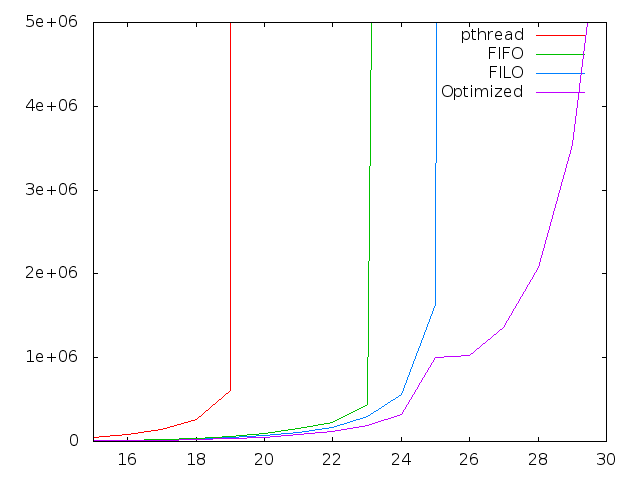
\includegraphics[width=\textwidth]{img/graph_comparaison}
\caption{Temps en millisecondes d'exécution de \textit{fibo(i)}}
\end{figure}

Ces résultats ont été obtenus sur une machine virtuelle avec un processeur Intel i5 2.53GHz tournant sous distribution Debian avec une RAM de 500Mb. Les asymptotes verticales montrent les valeurs de $i$ pour lesquelles les processus ont été tués par le \textit{Out of Memory Killer}.
\\

Le graphe montre bien que, lors d'un parcours quelconque de l'arbre d'appel, la complexité en mémoire est rapidement trop importante. L'ordonnancement optimisé de Fibonacci minimise le nombre de threads en mémoire à la hauteur de l'arbre ce qui permet de calculer des valeurs beaucoup plus grandes, jusqu'à \textit{fibo(40)} en environ 13 minutes. Globalement, la bibliothèque développée s'exécute plus rapidement que \texttt{pthread} puisqu'elle n'effectue pas de changements de contexte noyaux.
\\